\documentclass[useAMS,usenatbib]{mn2e}

% A Monthly Notices of the Royal Astronomical Society sample TeX file.
% The teX file has had all publication information removed and been left intentionally blank
% Created by: Martyn Bristow, M.Bristow@2007.ljmu.ac.uk, http://martynbristow.co.uk
% Edit this file to suit your needs, but be careful not to remove something important
% I have added sample images, tables and equations to help you if your don't know how to write them in LaTeX and to make your life easier.

\usepackage{graphicx}
\usepackage{float}
\usepackage{amsmath}
\usepackage{amssymb}
\usepackage{cite}
\usepackage{natbib}
\usepackage{xcolor}

\def\aap{Astronomy \& Astrophysics}
\def\apj{The Astrophysical Journal}
\def\mnras{Monthly Notices of the Royal Astronomical Society}

\usepackage{newtxtext,newtxmath}
\usepackage[T1]{fontenc}
\usepackage{ae,aecompl}

\newcommand{\red}[1]{{\color{red} #1}}

%%%%%%%%%%%%%%%%%%% TITLE PAGE %%%%%%%%%%%%%%%%%%%


\title[SL Challenge]{Strong Gravitational  Lensing Finding Challenge}

\author[R. B. Metcalf {\it et al.}]{
R. Benton Metcalf,$^{1}$\thanks{E-mail: robertbenton.metcalf@unibo.it} R\'emi Cabanac,$^2$ 
Alessandro Sonnenfeld,$^5$ \\
% List of institutions
$^{1}$Department of Physics and Astronomy, Universit\`a di Bologna, viale Berti Pichat 6/2, 40127 Bologna, Italy \\
$^{2}$ IRAP, University of Toulouse, CNRS, UPS, France.\\
$^{5}$Kavli IPMU (WPI), UTIAS, The University of Tokyo, Kashiwa, Chiba 277-8583, Japan\\
}

\begin{document}

\date{Accepted . Received ; in original form }

\maketitle

\label{firstpage}

% Abstract of the paper
\begin{abstract}

\end{abstract}

\begin{keywords}
gravitational lensing -- cosmology 
\end{keywords}


\section{Introduction}

some numbers about future surveys

\section{The Challenge}

\section{the simulations}

\section{lens finding methods}

This section contains short descriptions of the lens finding methods that were used in 
the challenge.  Each subsection refers to a team which gave a separate entry.

\subsection{GAHEC IRAP}

\begin{figure}
 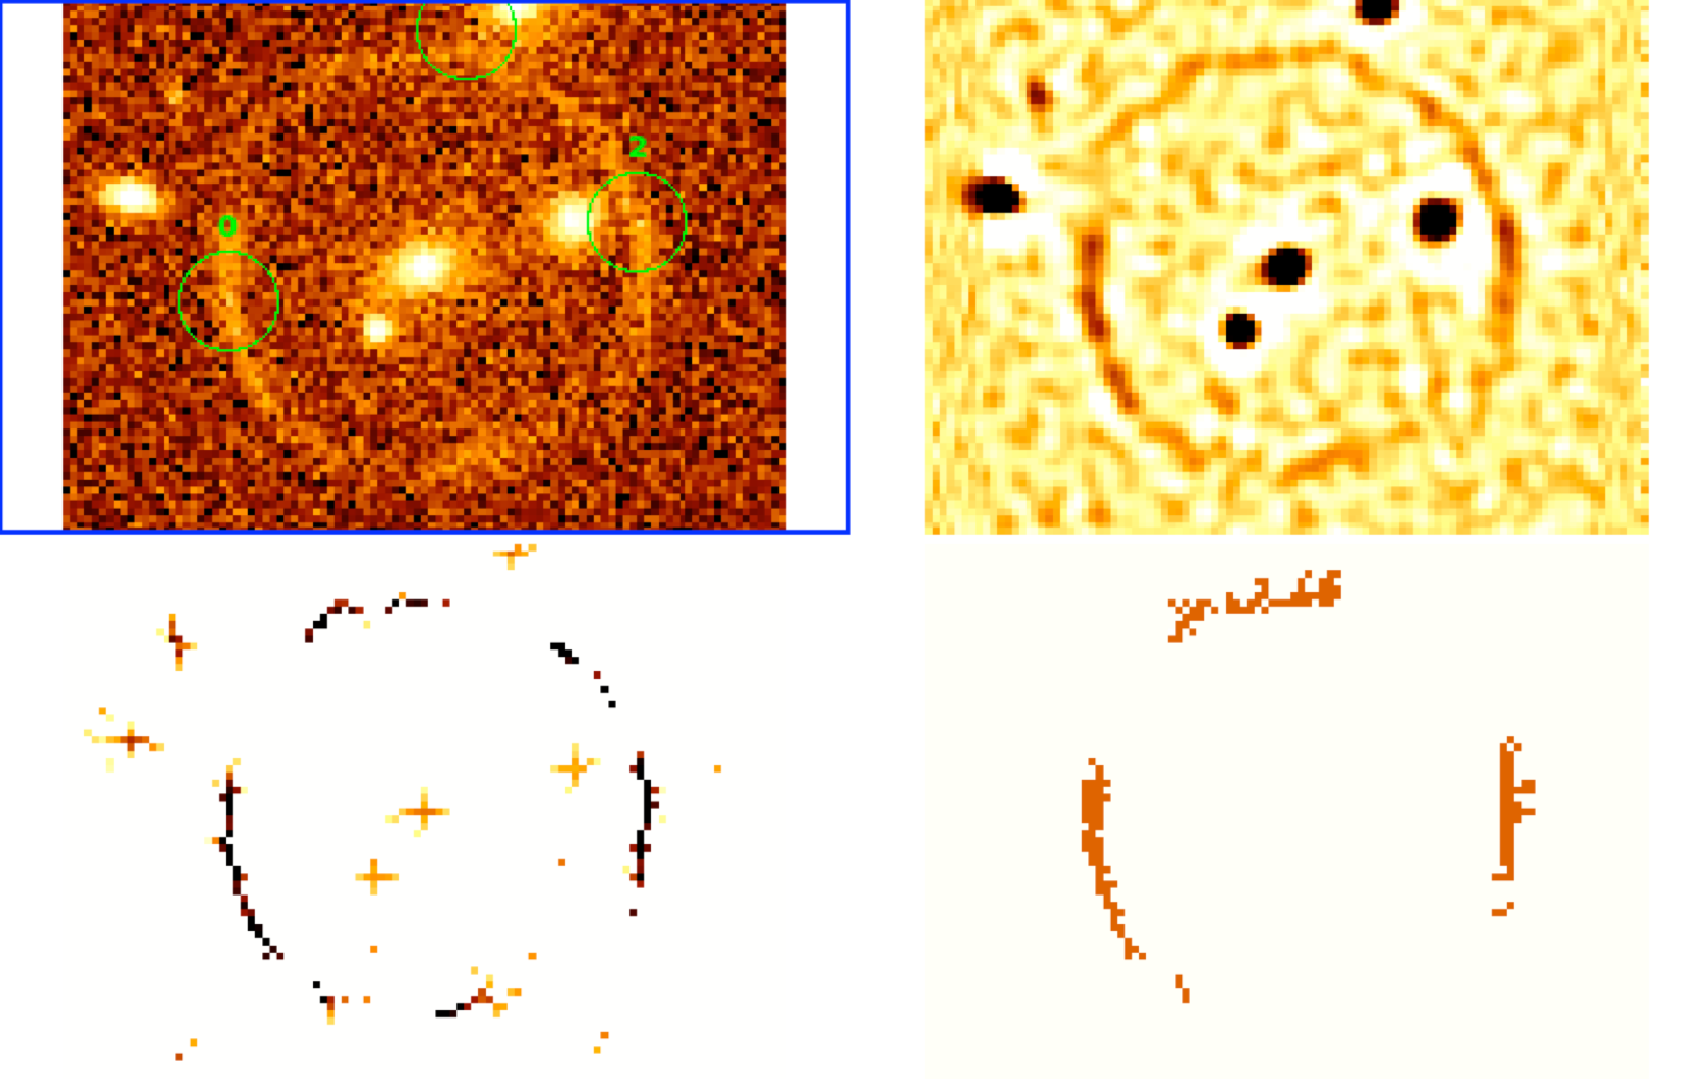
\includegraphics[width=\columnwidth]{Cabanac/arcmethod.pdf}
 \caption{ (GAHEC IRAP) From top-left to botton right, 1) a simulated arc extracted from SL challenge in which an tunned Arcfinder selects 3 candidates (green circles), 2) the smoothed image on which pixelwise elongation is computed, 3) the resulting elongated pixels after thresholding, 4) the set of pixels selected for the computation of arc candidate properties. }
 \label{fig:Cabanac}
\end{figure}

Arcfinder \citep{2006astro.ph..6757A,2007A&A...461..813C,2012ApJ...749...38M} is a fast linear method that computes a pixelwise elongation parameter (ratio of first-order moments in a n-pix window oriented in proper reference frame) for all pixels of mexican-hat-smoothed FITS images. Arcfinder then extract contiguous pixels above a given background and computes the candidate arcs length, width, area, radius of curvature and peak surface brightness. A final thresholding is set to maximize purity over completeness on a few typical arcs of the dataset.
For the current SL challenge, arcfinder was tunned to detect long and narrow arcs, and was optimized on a subset of 1000 simulated images with a grid covering a range of elongation windows and arc areas.  A python wrapper allows users to change parameters in a flexible way and run the arcfinder C code as a linux line command. Arcfinder took a couple of hours to run on the entire dataset with some overheads due to the dataset format. The code is publicly available at https://github.com/rcabanac/arcfinder.

\red{Reference to figure \ref{fig:Cabanac}?}

\subsection{YattaLens Lite (Alessandro Sonnenfeld)}
YattaLensLite is a simpler version of the algorithm YattaLens (Sonnenfeld et al. in prep.), modified to meet the time constraints of the challenge.
YattaLensLite subtracts a model surface brightness profile describing the lens galaxy from the $g$-band image, then runs SExtractor to detect tangentially elongated or ring-shaped objects, which are interpreted as lensed images.
In the ground-based challenge, the model lens surface brightness profile is obtained by taking a rescaled version of the $i$-band image.
The difference in color between lens and source usually allows the lensed images to still be detectable after the lens subtraction process.
However in order to avoid subtracting off the lensed images in systems with similar colors between lens source, we radially truncate the model lens surface brightness.
at the smallest radius between the position where the surface brightness is comparable to the sky background level or the position of a positive radial gradient in surface brightness, if detected.

In the space-based challenge it is not possible to separate lens and source based on color, because only data in one band is provided. The lens light model then is produced by taking a centrally-inverted image and then using the same truncation prescription used with ground-based data. The central inversion step is taken to reduce the chances of subtracting flux from lensed images, which are in general not centrally symmetric as opposed to typical lens galaxies.

In the full version of YattaLens, a lens modeling step is performed to improve the purity of the sample. However, such a procedure is too time consuming and was not performed in this challenge.

\section{results}

\section{Conclusions \& discussion}

It is clear that the robustness of lens finders against falsely classifying unusual galaxies as lenses was not adequitely tested in this challenge.  Some of the methods which appear overly conservative in this test might be better at avoiding false positives in real data.  This can be seen as a form of overfitting to the test set.
In future challenges we wish to concentrate on this aspect of the problem.

Human inspection was the only method to find the jackpot lens

\section*{Acknowledgements}

AS was supported by World Premier International Research Center Initiative (WPI Initiative), MEXT, Japan.
RBM's research was partly part of project GLENCO, funded under the European Seventh Framework Programme, Ideas, Grant Agreement n. 259349.

%%%%%%%%%%%%%%%%%%%%%%%%%%%%%%%%%%%%%%%%%%%%%%%%%%
%%%%%%%%%%%%%%%%%%%% REFERENCES %%%%%%%%%%%%%%%%%%

\bibliographystyle{mn2e}
\bibliography{references}

%%%%%%%%%%%%%%%%%%%%%%%%%%%%%%%%%%%%%%%%%%%%%%%%%%
%%%%%%%%%%%%%%%%% APPENDICES %%%%%%%%%%%%%%%%%%%%%

\appendix

\label{lastpage}
\end{document}
